\section{Results and discussion}

%------------------------------------------------

\begin{frame}
    \frametitle{Comparison of model performance}
    \vspace{3mm}

\begin{table}
        \centering
        \captionsetup{justification=centerlast}  % Configura el caption centrado
        \begin{tabular}{lcc}
        \hline
        \textbf{Model} & \textbf{Accuracy} & \textbf{F1-score} \\
        \hline
        Only Radiomic & 0.62 & 0.45 \\
        Radiomic + Reduced clinical data & 0.56 & 0.42 \\
        Radiomic + Full clinical data & 0.75 & \cellcolor{green!25} \textbf{0.78} \\  % Mejor F1-score en verde
        Radiomic + Multigenic & 0.81 & 0.74 \\
        All (Radiomic + Full clinical + Multigenic) & 0.75 & 0.60 \\
        Only full clinical data & 0.67 & \cellcolor{red!25} \textbf{0.40} \\
        Only Multigenic & 0.75 & \cellcolor{red!25} \textbf{0.40} \\  % Peor F1-score en rojo
        \hline
        \end{tabular}
        \vspace{3mm}
        \caption{Performance results for the different models based on accuracy and macro F1-score.}
        \label{tab:model_performance}
    \end{table}

    \vfill 
\end{frame}

%------------------------------------------------

\begin{frame}
    \frametitle{Detailed performance of the best model}
    \vspace{3mm}

    Due to the strong performance of the Radiomic + Full Clinical Data model, we consider it relevant to explore its performance using the confusion matrix from the test set.

    \vspace{1mm}

    \begin{figure}
        \centering
        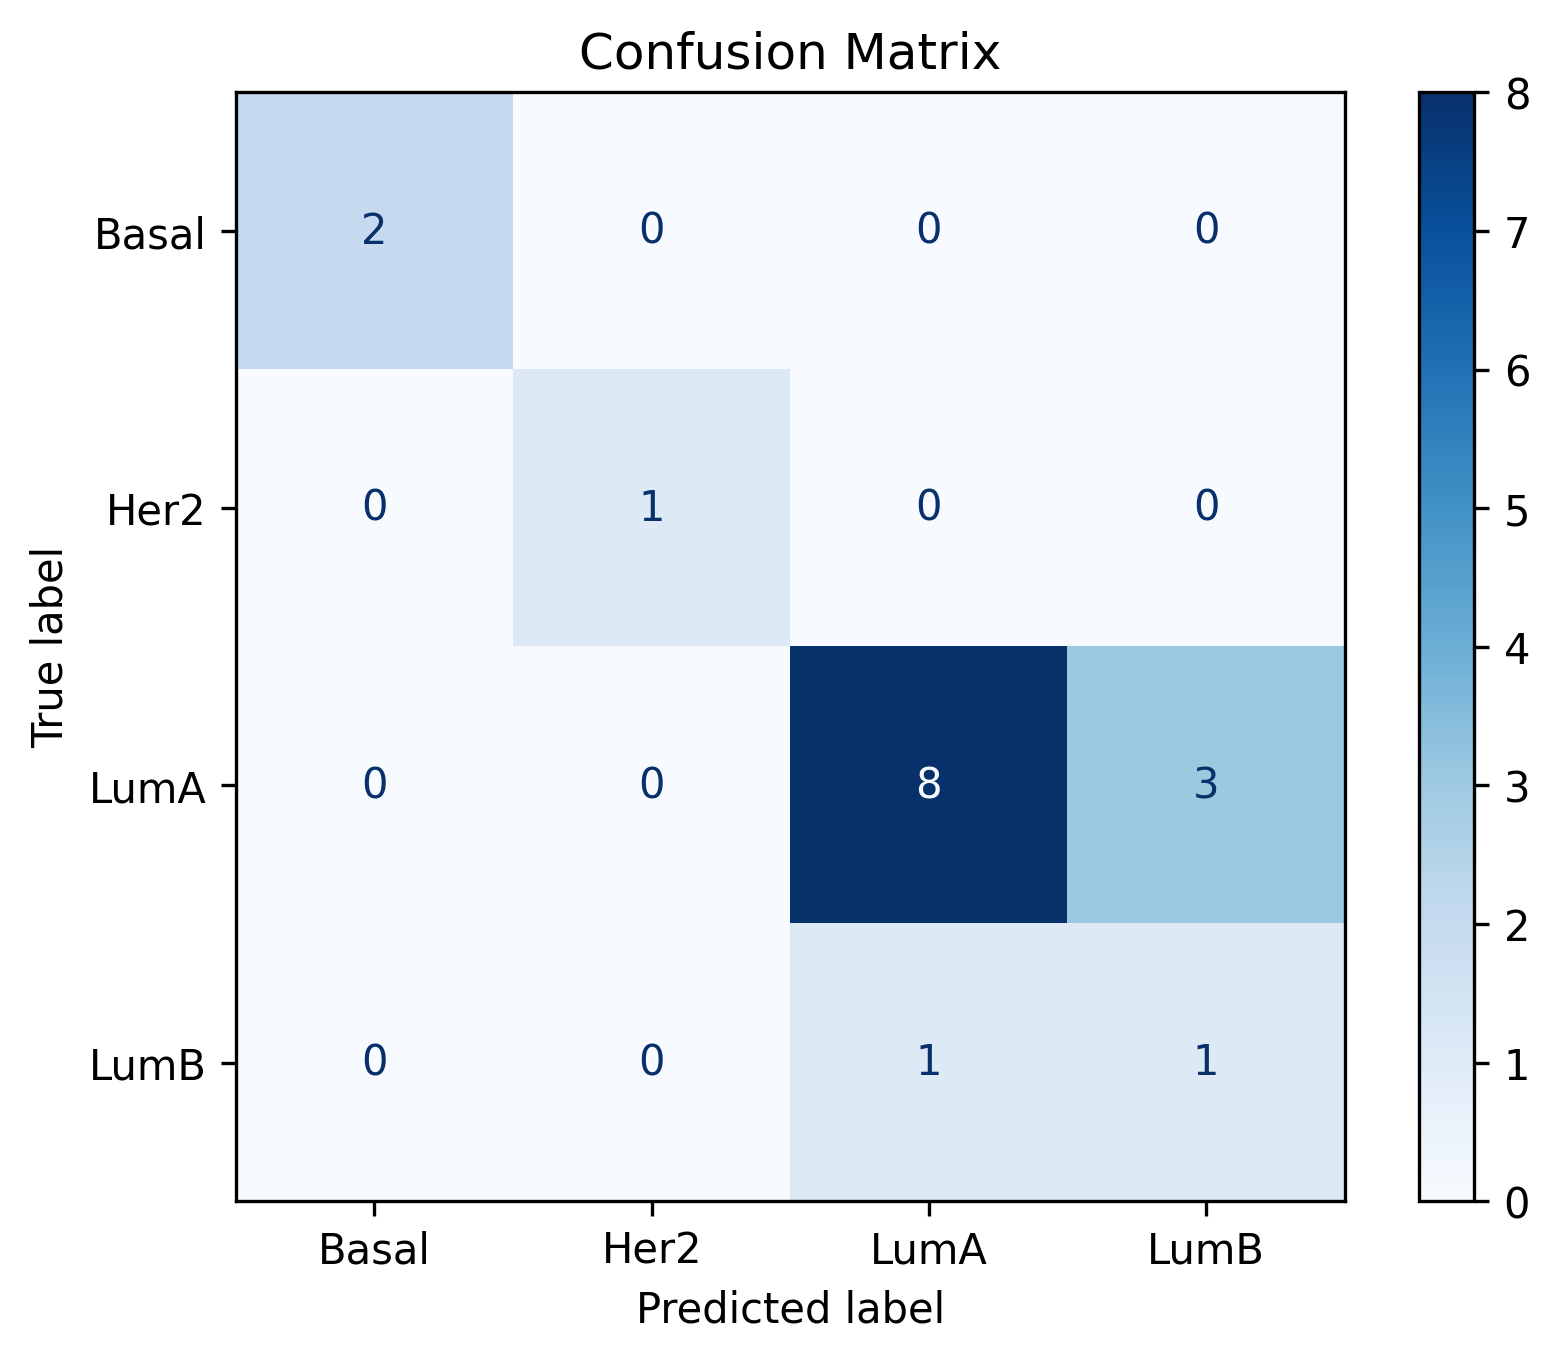
\includegraphics[width=0.6\linewidth]{confusion_matrix}
        \label{fig:confusion_matrix}
    \end{figure}

    \vfill 
\end{frame}